\section{Path Planner} \label{sec:navigator}
\subsection{Principle of motion planning for a sailing boat} \label{sec:intro_principle}
Due to the nature of every sailing vessel, \textsc{Avalon}'s manoeuvrability is
limited in relation to wind direction. Additionally, due to the non-holonomic
properties of a sailing vessel, it is not possible to change the heading on the
spot immediately.  The trajectory tracker (see section \ref{sec:skipper}) has
to keep that in mind and operate in a way that allows a certain space to make
heading changes. For the implementation of a navigation algorithm, these
constraints imply that using accurate wind information for every calculation is
essential.
 
\subsection{Literature Research}
%
Path planning in the naval industry is not a new topic. For many years,
commercial ships have used weather forecasts to generate an optimal path with
respect to speed or bypassing bad weather situations. For sailing ships,
commercial solutions by companies like \textsc{B \& G} or \textsc{Northstar}
exist, but do not offer any possibility to be integrated into our embedded
system. Looking at different navigation and routing strategies, two
fundamentally different ideas emerge: Roland Stelzer \cite{stelzer2008}, who
has published his approach also for implementation in an autonomous sailing
boat, projects the speed vector on the target direction and tries to find a
sailable heading that maximises that projected speed vector. Although in small
scale it might find a good and fast path, this approach is not sufficient when
it comes to larger search areas with obstacles and additional inputs like
weather forecasts.

The other approach is to use grid based path planning algorithms that allow us
to generate optimal solutions considering the path from start to goal and
enable the integration of specific constraints (see section
\ref{sec:intro_principle}).

\textit{Breadth first method} and \textit{Depth first} are both based on a very
simple principle and serve as archetypes for many important algorithms
\cite{cormen2001}, but may result in very long running time. \textit{Dijkstra}
on the other hand is a directed search \cite{lavalle2006} and guarantees
optimal results. A* is a modified version of \textit{Dijkstra} that also
considers the heuristic distance estimate of the path from current position to
the destination \cite{hart1968}, which makes it more directed than
\textit{Dijkstra}. One of the problems of grid-based planning algorithms is
that the angles are artificially constrained. The Theta*-Algorithm
\cite{nash2007} deals with that handicap and produces more realistic looking
paths than A* or even smoothed A*. A further extension of A* is D*
\cite{stentz1995}, which incorporates dynamic changes (i. e. moving obstacles)
along the path and does not require to replan the whole path from current
position to destination anymore.

The proposed approach uses a simple A* algorithm which is modified to comply
with all the sailing constraints. It must also be noted that there is few
computation time constraints for a sailing boat crossing the Atlantic ocean.
Even if path planning requires a handful of minutes, this is still an
acceptable behaviour.
%
\subsection{Planning Strategy}
%
Considering the distance of about 4'200 nautical miles \textsc{Avalon} has to
sail on its journey across the Atlantic Ocean and its slow speed of
about 4 to 5 knots\footnote{1 knot is 1 nautical mile per hour}, it is essential to distinguish between a global and a local
planning. Global planning will be done by fixing way-points across the Atlantic
based on expert knowledge, weather and current analysis. The local planner will
then plan from current position to the next global way-point using wind data
from the on board sensor. The planning algorithm will be triggered and
controlled by a trajectory tracker (section \ref{sec:skipper}), which knows
exactly towards which way-point \textsc{Avalon} is sailing at the moment.
%
\subsection{Interfaces with the controller}
An important part of the software structure is the interface between the
navigation program and the control system (see section \ref{sec:sailor}). The main
reason why we decided to pass \textit{headings} instead of way-points from the
planner via the trajectory tracker to the controller, was that the planner calculates an optimal
path with respect to path duration for specific angles to the wind.
Drift that pushes the vessel off the trajectory will be handled by the controller,
a new calculation will only take place after the boat has a certain deviation
from the set trajectory (see section \ref{sec:skipper}).
\paragraph{Wind data}
The wind the local path planner uses is an average of the measurements over the last 90 seconds. The control system will then follow the received desired heading using a much more accurate wind direction that was averaged only over a period of 5 seconds (see section \ref{sec:sailor}). Figure \ref{fig:cleanwind} shows a comparison of the two different wind sets.
%
\begin{figure}
 \centering
 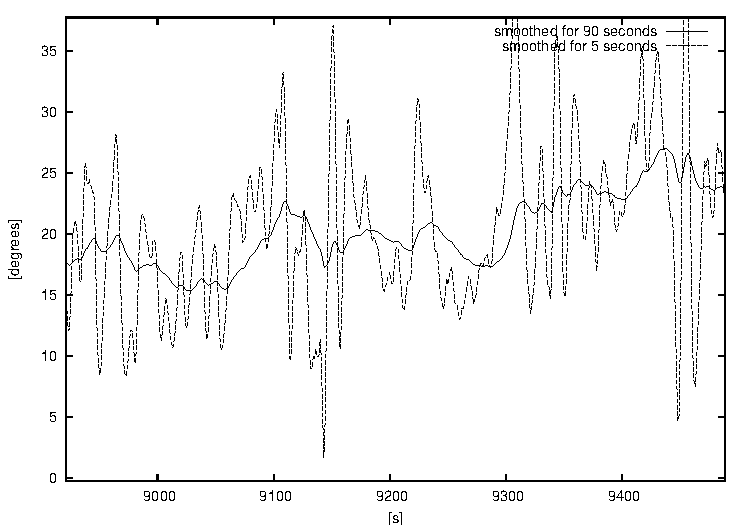
\includegraphics[width = 6.5 cm]{pics/paper_cleanwind.pdf}
 \caption{Differently filtered wind information}
 \label{fig:cleanwind}
\end{figure}

%
\subsection{Planning algorithm}
As explained earlier, \textit{Dijkstra}'s graph search is the basic algorithm
used to perform the path search. Starting at an initial grid-point, the algorithm expands over the whole field until the final grid-point has been reached. Every evaluated grid-point will be assigned a certain cost, a time estimate of how long it will take the boat to sail from the initial grid-point to the point that is currently being evaluated. The final optimal path is then determined by always following the neighbor with the lowest costs from the final to the initial grid-point. 

To be able to allocate costs for ship movements, i. e. moving from one grid-point to a neighbor, we work in 3 dimensions, with $x$ and $y$ for the geographic position
and $\theta$ for the heading of the boat at that position. To get sailable and
reasonable results, the following costs have been implemented additionally:
%
\begin{itemize}
\item Sailing-Time from start node
\item Estimated sailing time to the end node (heuristic)
\item Cost for heading changes
\item Cost for manoeuvres (tack and jibe)
\item Cost for offset from the straight connection between start and end node (tunnel cost).
\end{itemize}
%
\subsubsection{Grid compatible coordinate system}
To represent GPS points on a map, a coordinate transformation is necessary. Since we plan only for short distances ahead of us (local planning), we can use a very simplified transformation into meter coordinates 
\begin{equation}
\begin{array}{l}
 x = R_E \cdot \cos\left( \text{lat}\right) \cdot \dfrac{\pi}{180\, deg} \cdot \text{lon}\\
\\
 y = R_E \cdot\dfrac{\pi}{180\, deg}\cdot \text{lat}
\end{array}
\end{equation}
where $R_E$ is the earth radius, lon and lat the GPS coordinates in degrees. This transformation assumes a flat water surface \cite{stelzer2008}. In order to initialise the local map as small as possible, the algorithm places the origin as close as possible to either start or target coordinate. 
%
\subsubsection{Polar diagram}
In order to calculate the boat speed for a specific angle to the wind, a polar
diagram\footnote{In boating term, the polar diagram gives a boat velocity  as a
function of its  heading to the wind and the wind velocity} of \textsc{Avalon}
is needed.  Since creating a detailed diagram for our boat would require
constant wind and wave conditions over a long time, we created a polar diagram
based on existing diagrams for bigger vessels. Testing has shown that we get
reasonable results by restricting the sailable \textit{angle to the wind} to
the area between $45^o$ and $160^o$ (see figure \ref{fig:courses_to_wind}).
%
\subsubsection{Heading}
\hide{
% This is too much inmplementation dependent
We assume a 24 neighbour grid throughout this paper, which allows to have
sixteen different headings available for sailing. Another advantage of being
able to expand to the second but next neighbour-grid is the fact that it reduces
the number of way-points, since one grid node is skipped.
\subsubsection{Connectivity List}
In theory, every heading change is possible with a sailing boat. However, to
make the algorithm faster, we have constricted the biggest possible change of
heading to $90^o$. The areas that are not sailable due to the wind direction
are between $\pm45^o$ to wind direction for sailing upwind and $\pm160^o$ to
wind direction for sailing downwind (see figure \ref{fig:courses_to_wind}).
%
}
In order to limit the size of the 3D grid used in this paper, we use a
discretisation of the possible boat heading into 16 possible headings. In usual
2D grid-based path planning, transition from one cell to its 8 neighbours is
considered. This results in only 8 possible changes of orientation. By
considering a neighbourhood of 24 cells (8 cells around the starting cell, plus
16 cells one cell further), we can reach 16 different heading changes in one
transition. This leads to smoother paths and smaller number of way-points on the
final path.

We further reduce the computational complexity of the planner by considering
that the maximum change of heading in one transition is $90^o$. This
restriction is consistent with the experience of human skippers. 
%
\subsection{Cost Factors}
\subsubsection{General Costs}
The general aim of this algorithm is to find the shortest path for a sailing vessel to go from point $A$ to point $B$. The general cost we give for every movement is therefore \textit{sailing time to the next node}, calculated by equation \ref{eq:navi_timecost}. The speed solely depends on the angle to the wind and the wind speed. 
\begin{equation}
 \text{sailing time} = \frac{\text{distance to next node}}{\text{speed}} 
\label{eq:navi_timecost}
\end{equation}
\subsubsection{Heuristic Estimate}
The heuristic estimate is used to evaluate the remaining time to the goal.
According to \cite{lavalle2006}, the only constraint on the heuristic is that
it has to underestimate the real cost of the remaining path. For simplicity sake, the
heuristic returns the time it would take to sail to the goal at an exaggerated speed of 10 knots. More complicated options have been considered, but none of them provided well defined behaviour in all situations.

\subsubsection{Turning Cost}
To generate paths as smooth as possible, the algorithm places costs $C_{\text{new}}$ for heading changes, using a simple linear factor $f$ in equation
\begin{equation}
 C_{\text{new}} = f \cdot \vert \theta_{\text{curr}} - \theta_{\text{new}} \vert  
\label{eq:navi_turningcost}
\end{equation}
where $\theta_{\text{curr}}$ and $\theta_{\text{new}}$ are the respective headings. 
%
\subsubsection{Cost for Tack or Jibe}
By giving a certain cost for tack or jibe, we can indirectly control the number
of manoeuvres \textsc{Avalon} sails.  The principle is very simple, we check if
the sign of $(\theta_{\text{curr}} - \text{winddirection})$ and $(\theta_{\text{next}} -
\text{winddirection})$ is the same. If it is different, an additional cost will be
added to the total cost.
%
\subsubsection{Tunnel cost}
In order to favour paths that stay closer to the straight line path, we
allocate costs increasing with the distance from the direct connection of start
and target node. It has proved best to increase the cost only little for the
areas in the middle of the tunnel but increase it abruptly when closing in on
the borders. 
%
\subsubsection{Obstacle avoidance} 
To avoid islands and coastal regions, the algorithm gives extremely high costs
for passing prohibited terrain. To locate these areas, it parses information
from a map.\\
To avoid commercial ships on the Atlantic, \textsc{Avalon} can receive AIS
signals from most ships travelling over the Atlantic. Knowing ship speed,
direction and current position, our algorithm will place no-go areas around potential collision locations to make sure to bypass them.
%
% we had that already in chapter nav_strategy:
\hide{
\subsection{Trajectory tracker} \label{sec:skipper}
The trajectory tracker has mainly two important tasks:
\begin{itemize}
 \item Triggering the local planner
 \item Calculating a desired heading for the control system
\end{itemize}
\subsubsection{State machine}
To manage the different tasks, the trajectory tracker can switch between different states:
%
\paragraph{Standard Navigation}
If not approaching a target or buoy, this state generates headings for the control system, going from way-point to way-point.
If the wind changes more than $20$° or if the ship distances itself from the current trajectory for more than a predefined distance, a new calculation will be initiated. 
\paragraph{Goal Approach}
If approaching a target position, the trajectory tracker will always send a heading that is directing exactly towards that point.
\paragraph{Buoy Approach}
This is a state designed especially for short course racing. Due to regulations that always require a port-side surrounding of the regatta buoys, this state will - when approaching a buoy - always write a heading that will lead the boat around the buoy.
\paragraph{New Calculation}
In this state, the trajectory tracker manages and supervises the new calculation. After having checked that the new way-points have been stored, it switches back to \textit{Standard Navigation}
}
%
%
\subsection{Tests and Discussion}
\subsubsection{Testing environment}
Most tests and parameter optimization was done by visualising the generated
path on screen and discussing its quality. Figure \ref{fig:navi_path}
shows two calculated path examples, both having to pass an obstacle and dealing
with difficult wind direction like upwind and downwind. Analysis has shown that the addition of a tunnel cost is redundant since the heuristic estimate also favours paths that are close to the direct connection of {\em start} and {\em target} node. Although adding an artificial tunnel cost might not always result in optimal path solutions, we used the tunnel for safety reasons to make sure that the vessel never sails beyond predefined boundaries. 
\hide{
% In case of present obtacles, this is not always optimal.
\paragraph{Initial and final Heading}
Our initial motion was to set the current boat heading as $theta$ at the START
node. In case the TARGET was exactly in the opposite direction, the algorithm
then proposed a turn, which took about two to three way-points. Tests on the
water showed that this was not optimal at all and the manoeuvre cost us a lot of
time. We then set the START $theta$ directly towards the TARGET, which produced
much better results. One disadvantage is that the boat might sail away too far
from the starting point in case of long calculation time without receiving the
new heading. After calculation has finished, the trajectory tracker would then
notice the incoherence and trigger a new calculation. 
}

Another important and not yet solved problem is the final heading at the target
node that has to be known in order for \textit{Dijkstra} to start the search. At the
moment the algorithm chooses a final heading that is as close as possible to
the direct heading of a straight line from start to destination but always
differs at minimum $45^o$ from the wind direction. This usually produces good
results but it does not take obstacles into account which means that sometimes
an additional, unnecessary turn is produced. 

In practice, this issue will be solved by starting planning a new path before
completing the execution of the current one.


\begin{figure}[htb]
  \centering
  \subfloat[Upwind]{\label{fig:navi_upwind}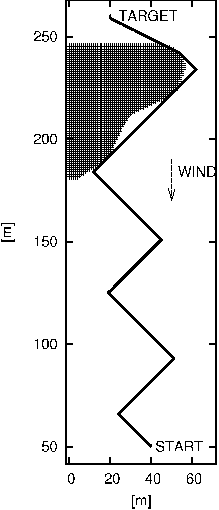
\includegraphics[width=2.7 cm]{pics/paper_kreuzen2.pdf}} 
  \hspace{1cm}
  \subfloat[Downwind]{\label{fig:navi_downwind}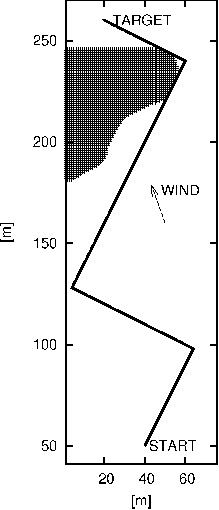
\includegraphics[width=2.7 cm]{pics/paper_downwind2.pdf}}
  \caption{Path examples for upwind and downwind sailing with obstacles}
  \label{fig:navi_path}
\end{figure}
